Di-quadraphonic -- post quarantine -- private installation, interpreted the 26th and the 27th of June, 2020 in Kr\aa kstad.

\bigskip

\noindent \textbf{{\large Presentation/Concept}}
\hrulefill

\bigskip

The performance requires four suspended `prepared' guitars\footnote{Inspired by the work of Alexander Refsum Jensenius -- see figure \ref{arj} (a). \\ \href{https://www.arj.no/2017/09/11/sverm-resonans/}{\scriptsize{\texttt{https://www.arj.no/2017/09/11/sverm-resonans/}}}
} with vibrating speakers inside the guitar boxes fixed as sound post of violins, inside a quadraphonic space using then four `normal' speakers -- see figure \ref{dpan}.

This composition plays on three layers, which are mixed and interpreted as an improvisation through the SuperCollider GUI -- see figure \ref{hk}. Hence, the duration is \textit{ad libitum} and should be managed as an installation, playing currently the `birdscape' in guitars as a `standby' state. 

The mix concerns the layers as such and the balance between the guitares and the speakers.

 \begin{figure}[hbt]
\begin{center}
	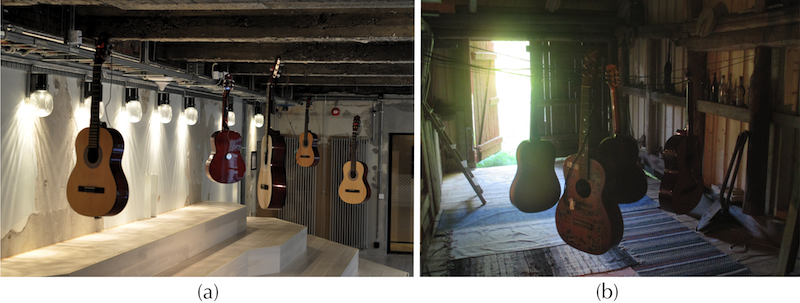
\includegraphics[width=\textwidth]{img/6757}		
\caption{(a) \textit{Sverm-resonans}, installation at the Ultima Contemporary Music Festival in 2017 by Alexander Refsum Jensenius. (b) \texttt{105A1208} installation in the shed -- Kr\aa stad, June 2020.}
\label{arj}
\end{center}
\end{figure}

 \begin{figure}[H]
\begin{center}
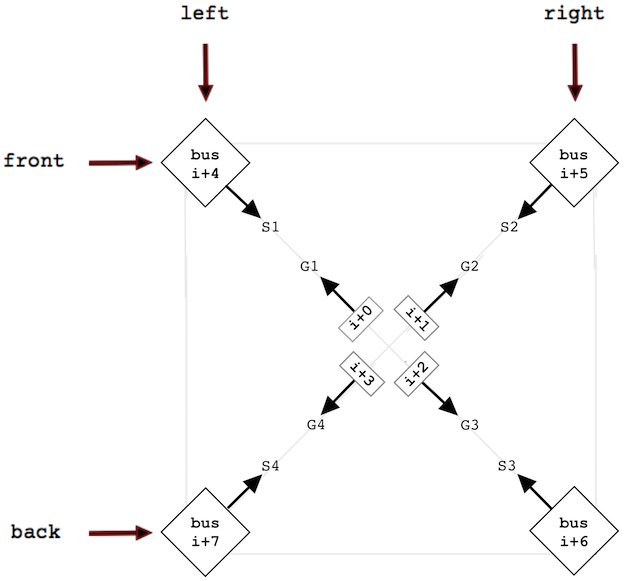
\includegraphics[scale=3.5]{img/6644}
\caption{`Di-quadraphonic' disposal in the shed -- \texttt{S} $\rightarrow$ Speaker, \texttt{G} $\rightarrow$ Guitar.}
\label{dpan}
\end{center}
\end{figure}

\begin{itemize}[leftmargin=0.4in]
\item \textbf{Layer I} : \textsc{`Birdscape'} 
\item \textbf{Layer II} : \textsc{Fractal} $\rightarrow$ on the rhythm analysis of the `birdscape' -- involved the command line \textsl{enkode} ($\rightarrow$ see \ref{enk}) for the analysis as initial data, the Common Lisp libraries N3 (function \texttt{differential-vector} $\rightarrow$ see \ref{motrec}) and \textsl{cl-mst} (functions \texttt{rhizome-degree} and \texttt{boruvka} $\rightarrow$ see \ref{amst}) -- as MDS $\rightarrow$ see \ref{mds}. 
\item \textbf{Layer III} : \textsc{Formantic Wind} 
\end{itemize}

\bigskip

\noindent \textbf{{\large Description}}
\hrulefill

\bigskip

  \textbf{\textit{a/} MDS }
  
  \smallskip
  Generating rhythmic patterns as Musical Data Score from the `birdscape' analysis.
  
 \begin{enumerate}
\item \textsl{enkode} analysis
 
\begin{lstlisting}[basicstyle=\footnotesize\ttfamily,language=Bash]
enkode -I 3 birdscape.wav > data.txt
\end{lstlisting}

\item generating MDS -- require package N3 and \textsl{cl-mst}
\begin{lstlisting}[basicstyle=\footnotesize\ttfamily,language=Lisp]
(defparameter *DATA* (mapcar #'N3::string-to-list 
   (N3::read-text-lines "data.txt")))
(defparameter *SEQ* (loop for i in *DATA* collect 
   (list (car i) (caddr i))))
(defvar *N* nil) ;; number of events

(defun loop-rtm (seq n)
  (loop for i from 0 to (- (length seq) n) by n 
     collect (subseq seq i (+ i n))))
     
(dotimes (n 5)
  (setf *N* (+ 5 n))
  (N3::>data-file (format nil "mds/105A1408-~S.mds" *N*) 
    (let ((dat (loop for i from 0 to (1- *N*) 
           collect
	  (let* ((mds (N3::mat-trans (nthcdr i *SEQ*)))
		 (tmp (mapcar #'list (loop-rtm (car mds) *N*) 
			             (loop-rtm (cadr mds) *N*)))
		 (matrix (N3::differential-vector tmp nil 
		                         :result :diff-x))
		 (mst (cl-mst:boruvka (mapcar #'(lambda (x) 
		       (list (car x) (cadr x) 
		              ;; avoid zero distance
		              (+ 0.01 (caddr x)))) 
		          matrix)))
		 (len (1- (length tmp)))
		 (res (loop for iii from 0 to len 
			collect (cl-mst:rhizome-degree iii mst)))
		 (maxi (car (N3::ordinate res '>))))
	     (list maxi (nth (+ i (position maxi res)) tmp))))))
	(append (loop for i in dat append (cadr i)) 
	        (list (cons 2 (mapcar #'car dat)))))))
\end{lstlisting}
\end{enumerate}

\begin{figure}[hbt]
\begin{center}
	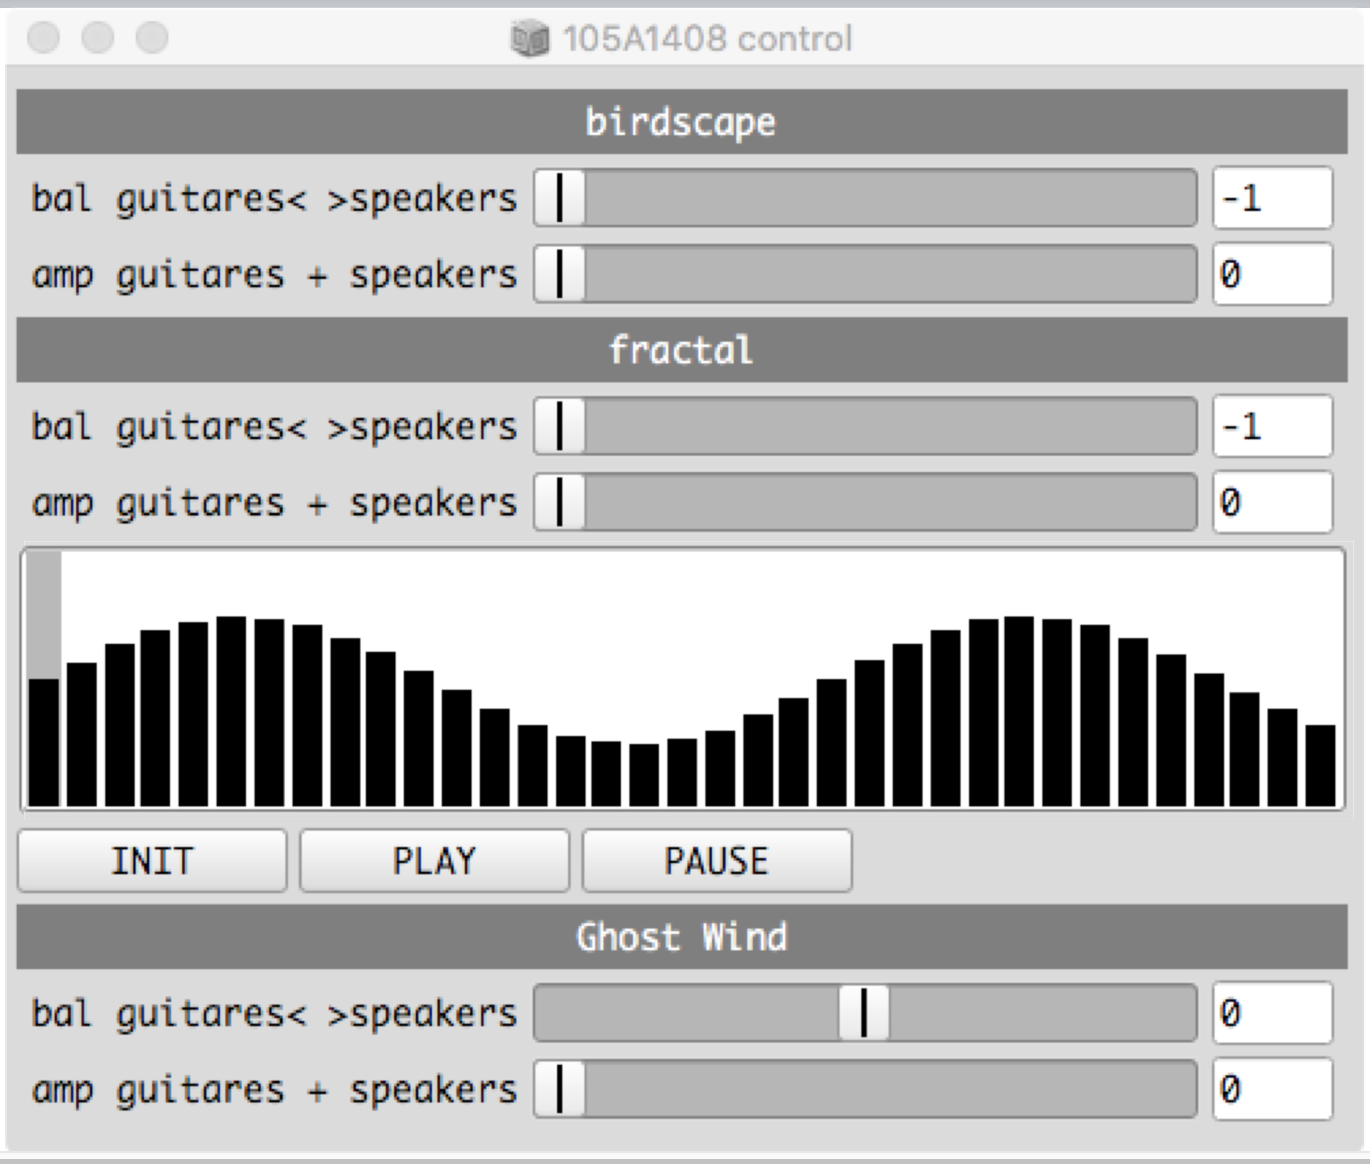
\includegraphics[scale=0.48]{img/9809}		
\caption{Playing and mixing \textit{in situ} with the SuperCollider GUI. Note that concerning the `fractal' layer, each slider represents a fractal recursivity from the right to the left, and the amount of the slider set how far is this recursivity.}
\label{hk}
\end{center}
\end{figure}

  \textbf{\textit{b/} Formantic wind}
  
  \smallskip 
  
  \begin{table}[htp]
\begin{center}
{\ttfamily
\begin{tabular}{|l|c|c|c|}
\cline{2-4}
    \multicolumn{1}{c|}{} & source (Hz) & range (Hz) & scale \\ 
    \hline 
    formant 1 (f1) & 312 - 750 & 300 - 750 & lin \\ 
 \hline
 bandwidth f1 & 90 & 45 - 180 & exp \\ 
 \hline
 formant 2 (f2) & 781 - 2031 & 750 - 2050 & lin \\ 
 \hline
 bandwidth f2 & 110 & 55 - 220 & exp \\ 
 \hline
 formant 3 (f3) & 2469 - 3187 & 2450 - 3200 & lin \\ 
 \hline
 bandwidth f3 & 170 & 85 - 340 & exp \\ 
 \hline
\end{tabular}}
\caption{Formant frequency ranges with their respective bandwidths, interpreted as an exponential range between half and the double of the initial value. The column `source' refers to the data in \citep{adc}.}
\end{center}
\label{default}
\end{table}%

	
	
	
	
